\section{Another Method For the Critical Years: Critodemus Begins with the Moon (12K,8P)}

An example: \Sun\xspace in \Aquarius, \Moon\xspace in \Leo, \Saturn\xspace in \Cancer, \Jupiter\xspace in \Gemini, \Mars\xspace in \Scorpio, \Venus\xspace in \Aries, \Mercury\xspace in \Pisces\footnote{\textit{Greek Horoscopes} dates the chart to February 11, 92 CE. No Ascendant is given by Valens so time unknown.} 

\begin{wrapfigure}[15]{R}{7cm}
\centering
\vspace{-20pt}
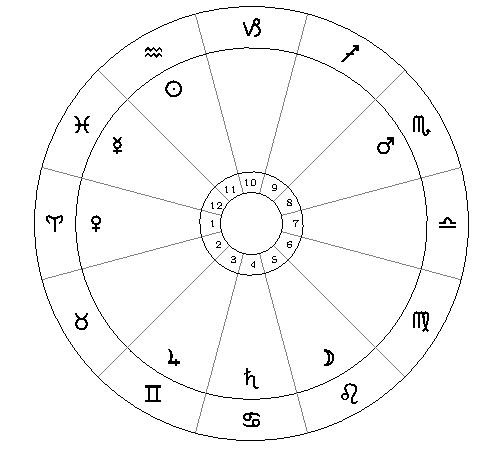
\includegraphics[width=.68\textwidth]{charts/5_12_1}
\caption{Chart 70 [V.12.1, GH L92, II]}
\label{fig:chart70}
\end{wrapfigure}

/235K/ The 12 years $<$are derived from$>$ \Mars’ distance of 4 signs
$<$from the \Moon$>$. The critical year is simple, because 4x4=16. (The squares are simple; the rectangular numbers are composite.) The 18 for \Venus\xspace is composite: 2x9. The 2 $<$is from \Leo$>$ to \Virgo, but no star is in \Virgo, so \Venus\xspace is 9 signs from the \Moon. \textbf{/224P/} If there were a star in \Virgo, it $<$\Venus$>$ would have returned because of the…

Since 3x6=18, we investigate this figure too. However, no star is in \Libra, the third sign $<$from the \Moon$>$, or in \Capricorn, the sixth.

Next 20 is composite, because 4x5=20, and 5x4=20. So \Mars\xspace in \Scorpio\xspace $<$the fourth sign$>$ is operative; no star is in \Sagittarius, the fifth sign.

3x7=21: no star is in \Libra\xspace $<$the third sign$>$, but the \Sun\xspace is in \Aquarius $<$the seventh$>$. So $<$the return$>$ is to the \Sun.

4x6=24: again \Mars\xspace is in \Scorpio\xspace $<$the fourth sign$>$, but no star is in \Capricorn\xspace $<$the sixth$>$.

25 is square, a simple number, but no star is in \Sagittarius\xspace $<$the fifth sign$>$.

3x9=27: no star is at the third interval, only \Venus\xspace in the ninth $<$\Aries$>$.

28 is composed of 4 (the return to \Mars) and 7 (the return to the \Sun).

4x10=40 and 5x8=40: this is associated with \Mars, because of the 4, and with \Mercury\xspace because of the 8.

$<$4x11=$>$ 44: this is associated with \Mars\xspace and \Jupiter.

 Sometimes several stars return to the same point together, as in the case of 40, because \Mars\xspace lies in the fourth sign and \Mercury\xspace in the eighth. If some star had been in the tenth and the fifth signs, they would also have returned together there.
 
 He says that outcomes will be more vigorous and obvious if the number of the year is the same as the number appropriate to the intervals between stars, as follows:
 
 \begin{table}[ht]
 \begin{center}
\begin{tabular}{l r l r}
\hline
\Saturn & 3 & \Jupiter & 10 \\
\Venus & 5 & \Moon & 13 \\
\Mars & 7 & \Sun & 18 \\
\Mercury & 8 \\
 \hline
 \end{tabular}
 \end{center}
 \end{table}

If the number and the interval coincide at the same star, the star will be operative in an operative sign. 

If the year-number does not coincide with any of the intervals applicable to the star, it will be inoperative in an inoperative sign. 

If one interval is found to be operative, but another interval does not occur in the subsequent years, the initial interval must be used until another is found. 

Using the preceding horoscope as an example: 28 is associated with \Mars\xspace and the \Sun\xspace <4 and 7>. 29 has no interval. 30 has 3, 5, 6, and 10: these signs too are empty. 31 again is not associated with any interval. Therefore \Mars\xspace and \textbf{/236K/} the \Sun, operative in the 28th year, control the succeeding years until the 32nd year, when \Mars\xspace (because of the 4) and \Mercury\xspace (because of the 8) have mutual returns. 

We will append the differences of the critical years according to the chronocratorships of the stars and their mutual returns to each other.

\begin{center}
\begin{longtable}{r p{0.8\linewidth}}
\hline
\textbf{Year} & \textbf{Critical Points and Results} \\
\hline
\endhead
1 & He will be sickly and anxious. \\
2 & He will be endangered by fluxes and convulsions. \textbf{/225P/} \\
3 & A critical point of \Saturn; precarious. \\
5 & Of Phosphorus $<$\Venus$>$; he will be weakened. \\
6 & A second critical point of \Saturn. \\
7 & The first critical point of \Mars: dangerous, involving fevers, bleeding, wounds, falls, ulceration, sword cuts. \\
8 & The first critical point of \Mercury; uncompounded. \\
9 & The first critical point of \Jupiter; the third point of \Saturn; dangerous. He will be sickly and and burdened with the ague and troubles of the bowels. \\
10 & The second point of \Venus. He will be ill because of surfeit. \\
12 & The fourth critical point of \Saturn. $<$He will die$>$ unexpectedly or because of moist matters. \\
13 & The first point of the \Moon; a difficult fever or seizures will occur; troubles of the insides or chest. \\
14 & The second point of \Mars; dangerous, troublesome. \\
15 & The fifth point of \Saturn, the third of \Venus; relaxing. \\
16 & The second critical point of \Mercury; compounded of cholera, bronchitis, and difficult convalescence. \\
18 & The second point of \Jupiter, the sixth of \Saturn, the first of the \Sun; very grievous. \\
20 & The fourth point of \Venus; generally safe; the diseases come from surfeit or exertion. \\
21 & The third point of \Mars, the seventh of \Saturn; difficult and dangerous. \\
24  & The eighth point of \Saturn, the third of \Mercury; difficult because of black bile and most syndromes. \\
25 & The fifth point of \Venus; compounded. \\
26 & the second point of the \Moon; dangerous. \\
27 & The third point of \Jupiter, the ninth of \Saturn; average. \\
28 & The fourth critical point of \Mars; precarious. \\
30 &The tenth point of \Saturn, the sixth of \Venus; generally safe. \\
32 & The fourth point of \Mercury; tiring. \\
33 & The 11th point of \Saturn; difficult. \\
35 & The fifth point of \Mars, the seventh of \Venus; dangerous and exposed to treachery. \\
36 & The fourth point of \Jupiter, the 12th of \Saturn, the second of the \Sun; grievous and dangerous. \\
39 & The third point of the \Moon, the 13th of \Saturn; precarious and dangerous. \\
40 & The eighth point of \Venus, the fifth of \Mercury; not grievous.
\textbf{/226P/42} The sixth point of \Mars, the 14th of \Saturn; grievous and dangerous. \\
45 & The fifth point of \Jupiter, the ninth of \Venus, the 15th of \Saturn. This critical point is called Stilbon. It is necessary to beware lest some infirmity of the foot occur at this time while \Mercury\xspace is operative in the nativity, because \Mercury\xspace brings dangers to the joints, sickness, life threatening and disgusting syndromes. \\
48 & The sixth point of \Mercury, the 16th of \Saturn; very grievous and dangerous. \\
49  & The seventh point of \Mars; sudden dangers through fevers, bleeding, \textbf{/237K/} and violent occurrences. \\
50 & The tenth point of \Venus; dangerous. \\
51 & The 17th point of \Saturn; it brings diseases, harm, and misfortune. \\
52 & The fourth point of the \Moon; not good. \\
54 & The 18th point of \Saturn, the sixth of \Jupiter, the third of the \Sun; grievous and full of danger. \\
55 & The 11th of \Venus; not bad. \\
56 & The eighth point of \Mars, the seventh of \Mercury; painful and bitter. \\
57 & The 19th point of \Saturn; the worst. \\
60 & The 20th point of \Saturn, the 12th of \Venus; precarious. \\
63 & The 21st point of \Saturn, the seventh of \Jupiter, the ninth of \Mars; the “Man-killer,” grievous and fatal \\
64 & The eighth of \Mercury; not especially bad. \\
65 & The fifth of the \Moon, the 13th of \Venus; a combination \\
66 & The 22nd of \Saturn\xspace … \\
69 & The 23rd of \Saturn; grievous \\
70 & The tenth of \Mars, the 14th of \Venus; difficult and grievous. \\
72 & The 24th point of \Saturn, the eighth of \Jupiter, the ninth of \Mercury; grievous and fatal. \\
75 & The 25th point of \Saturn, the 15th of \Venus; dangerous. \\
77 & The 11th point of \Mars; difficult and fatal. \\
78 & The 26th point of \Saturn, the sixth of the \Moon; grievous. \\
80 & The 16th point of \Venus, the tenth of \Mercury; a mixture. \\
81 & The 27th point of \Saturn, the ninth of \Jupiter; dangerous.\textbf{/227P/} \\
84 & The 28th point of \Saturn, the 12th of \Mars; difficult and malefic. \\
85 & The 17th point of \Venus; a combination. \\
87 & The 29th point of \Saturn; dangerous. \\
88 & The eleventh of \Mercury … \\
90 & The 30th point of \Saturn, the 18th of \Venus, the tenth of \Jupiter, the fifth of the \Sun; grievous. \\
91 & The 13th of \Mars, the seventh of the \Moon; difficult. \\
93 & The 31st of \Saturn; grievous. \\
95 & The 19th point of \Venus; not good. \\
96 & The 32nd point of \Saturn, the twelfth of \Mercury; difficult. \\
98 & The 14th point of \Mars; grievous. \\
99 & The 33rd point of \Saturn, the eleventh of \Jupiter; average. \\
100 & The 20th point of \Venus; not bad. \\
102 & The 34th point of \Saturn; grievous. \\
104 & The eighth of the \Moon, the 13th of \Mercury; not especially bad. \\
105 & The 35th point of \Saturn, the 21st of \Venus, the 15th of \Mars; difficult. \\
108 & The 36th point of \Saturn, the twelfth of \Jupiter, the sixth of the \Sun; fatal. \\
110 & The 22nd point of \Venus; not bad. \\
111 & The 37th point of \Saturn; precarious. \\
112 & The 16th point of \Mars, the 14th of \Mercury; difficult and dire. \\
114 & The 38th point of \Saturn; dangerous. \\
115 & The 23rd point of \Venus; a combination. \\
117 & The 39th point of \Saturn, the ninth of the \Moon, the 13th of \Jupiter; dangerous. \\
119 & The 17th point of \Mars; precarious. \\
120 & The 40th point of \Saturn, the 24th of \Venus, the 15th of \Mercury; fatal. \\
\hline	
\end{longtable}
\end{center}

\newpage
An example: \Sun, \Jupiter, \Mars\xspace in \Cancer, \Moon\xspace in \Libra, \Saturn\xspace in \Sagittarius, \Venus, \Mercury in
\Leo, Ascendant in \Gemini\footnote{\textit{Greek Horoscopes} dates the chart to July 17, 104 CE about 4 a.m.}.

\begin{wrapfigure}[15]{R}{7cm}
\centering
\vspace{-20pt}
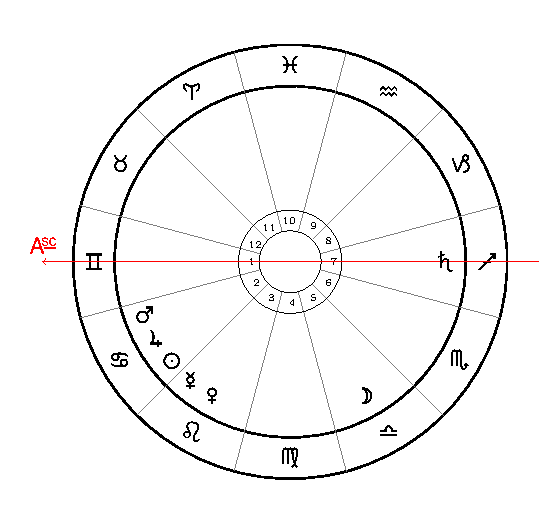
\includegraphics[width=.68\textwidth]{charts/5_12_2}
\caption{Chart 71 [V.12.2, GH L104, VII]}
\label{fig:chart71}
\end{wrapfigure}

The native died in his 54th year. The cycle was at the 18th critical point of \Saturn, the sixth of \Jupiter, the third of the \Sun, i.e. the mutual returns of these stars. The \Sun\xspace and \Jupiter\xspace
were found in the death-bringing month, \Sagittarius. In addition the \Sun, \Jupiter, and \Mars\xspace transmitted the 54th year from the $<$8th$>$ Place of Death $<$relative to the Lot of Fortune$>$ to \Saturn\xspace in Sagittarius. Such a transmission was grievous.

\textbf{/228P/} In every nativity it seems right to put the start of the critical points not just at the \Moon, but at all of the stars from whose $<$positions and nature$>$ the fatal times and life-threatening troubles can be determined. If the life-giving chronocrators take effect—this is determined by using these methods—the critical point will occur without any doubt. 

If the basis of the nativity has a continuation $<$of life$>$, \textbf{/238K/} but the critical point falls at that time, a crisis will occur with respect to actions and types of livelihoods: loss of rank, ruin, violence, convictions, shipwreck, trials, imprisonment, exile, anxieties, losses,
penalties, sudden dangers, threats, robbery, plus whatever crises arise in man’s life: injuries, diseases, amputations of the extremities, burns, cuts, illnesses, dangerous plots. 

If the stars which have critical points and which are mutually returning are found to be in opposition, beheld by malefics, and located out
of their own sect at the nativity, they indicate that the period will be precarious and troublesome. But if they are in an appropriate configuration, they weaken the onset of the crisis and make the critical point milder in its effects. 

The transmissions or receptions from signs of equal rising time must be considered active: from \Aries\xspace to \Pisces, from \Taurus\xspace to \Aquarius, from \Gemini\xspace to \Capricorn, from \Cancer\xspace to \Sagittarius, from \Leo\xspace to \Scorpio, and from \Virgo\xspace to \Libra. The same is true in reverse order.

These facts we have tested with sober reasoning and much careworn toil; we have expounded them with great labor for those who have the necessary intelligence. $<$We hoped$>$ to be able to equal both in
achievement and in fame what the sages of old accomplished when they devoted themselves to this art. But as it is, those who bastardize this science with fancy words and complicated schemes find it easy to
persuade not only those who are uninitiated into this art but also those who have something to boast of and who have a great reputation. Their success in persuading comes from the fact that their wizardry and effrontery is hard to grasp. Such men do not consider errors to be setbacks and they are successful in their brazenness, since they do not have blushes as the refutation of their ignorance. Instead they strut the stage like tragic or comic characters, walking in the ways of deceit, not of truth. 

But the man who has started with rules and theorems does not wish to bring disrepute on the knowledge which he gained with such difficulty, and so he leans on his experience as on a staff, \textbf{/229P/} and he answers slowly and hesitantly, and he is not driven $<$?$>$ from his purpose, because he considers that a mistake is worthy of exile or death, but that a success is the “toilsome heart \textbf{/239K/} of virtue.” This $<$error$>$ occurs with respect to the ignorant or those who do not precisely calculate the year or the hour.$<$?$>$

So it would be necessary for those wishing to hear with special confidence about the present or the future to judge carefully these men and to praise any of their deeds, so that the prognosticator, having grasped the precise effects of the angles and of the powerful places using specific numbers and a definite system, may forecast the truth.

For often (as I have said) not only have these deceptive men and their spiritual fathers falsified the times and wronged our science; I have learned this from my spiritual ancestors as well. But they do this
since they wished in one moment to hear things which are in accord with their desires and are mixed $<$with honor$>$, and to be involved with impossible things by means of some wicked magic art. After they have learned from the ignorant and done with enthusiasm what they should not have done, they then enjoy praise and honors, and repay their enemies: they revile honored men, the experienced $<$astrologers$>$, on the grounds that they cannot easily make forecasts nor compose treatises in detail. They do not know that the
details of each nativity are grasped only with much labor and investigation. Later thay fail in their expectations, and they not only repent and bring censure in a precarious and painful way on their own
falsehoods, but they also call this science “unreal” and consider its practitioners as enemies. Thus it happens that this science has been dishonored in the eyes of the public by a few men unworthy of it.

The end of Vettius Valens, Book V.

\newpage